\documentclass{article}

\usepackage[utf8]{inputenc}
\usepackage[frenchb]{babel}
\usepackage[T1]{fontenc}
\usepackage{amsmath}
\usepackage[cm]{fullpage}
\usepackage{multicol}
\usepackage{graphicx}

\author{Martin Janin}
\title{Modèle 3D d'un objet à partir de photographies: Extraction de silhouette}

\begin{document}

\maketitle

Le travail effectué est celui prévu. La majorité de l'étude à été concentrée sur la détection de contours. La segmentation de l'image obtenue étant effectuée par le procédé simple présenté par Baumgart.

\noindent\makebox[\linewidth]{\rule{\textwidth}{0.4pt}}
\vspace{-0.8cm}
\tableofcontents
\noindent\makebox[\linewidth]{\rule{\textwidth}{0.4pt}}

\bigskip
\bigskip

\begin{multicols}{2}

\section{Introduction}

Le travail consiste en l'implémentation complète d'un script d'extraction de silhouette en python. Celle-ci a entraînée une réflexion importante sur l'optimisation du programme, de la manière d'implémenter les différentes étapes jusqu'au choix des types et structures utilisés. On détaillera d'abord les choix d'implémentations avant de présenter succintement le procédé, trop complexe pour être completement expliqué ici.

\section{Choix d'implémentation}

La totalité du programme est écrite en python. Il comprend certaines commandes en bash afin de suivre l'évolution de l'utilisation de la mémoire vive.

Les modules utilisés sont :

\begin{tabular}{l p{5cm}}
	numpy & $\longrightarrow$ structure et opérations \\
	system & $\longrightarrow$ suivie de la mémoire \\
	matplotlib & $\longrightarrow$ tracés et affichage des images \\
	itertools & $\longrightarrow$ outils sur les générateurs \\
	time & $\longrightarrow$ suivie du temps d'execution de chaque étape
\end{tabular}

\subsection{Types et structures}

Le programme prend en entrée une image RGB de taille de l'ordre du mégapixel. Traiter des données de cette taille motive des choix qui ne sont pas habituels dans d'autres domaines de l'informatique.

\subsubsection{Type}

Le type retenu est le type float32 de numpy, conjugué naturellement au type complex64. C'est le meilleur choix pour plusieurs raisons :
\begin{itemize}
	\item Les opérations sur les flottant sont plus rapides que sur les entiers. En effet, les processeurs sont d'abord conçus pour effectuer des opérations sur des nombres flottants.
	\item Les 8 bits alloués à l'exposant du type float32 permettent un nombre maximal de $10^{256}$ ce qui évite tout dépassement de capacité.
	\item Il est bien plus aisé de normaliser une image de flottants puisque le type gère de lui même la perte de précision (contrairement aux entiers)
	\item Du fait des grandes complexités spatiales, il était impossible d'utiliser des flottants sur 64bits.
\end{itemize}

\subsubsection{Structure}

En ce qui concerne la structure adoptée, il s'agit des tableaux numpy, pour des raisons d'efficacité. On est amené à utiliser des tableaux à 5 dimensions, réparties comme suit :
\begin{itemize}
	\item Les 3\up{ème} et 4\up{ème} correspondent au plan de l'image : indexer par rapport à ces dimensions correspond à choisir un pixel.
	\item Les deux premières dimensions correspondent au voisinage de chaque pixel. Chaque pixel contient en effet tout son voisinage afin de pouvoir effectuer des opérations dessus.
	\item La 5\up{ème} dimension est celle des composantes. On manipulera en effet des images composites, à l'instar d'une image RGB, ce qui permet d'effectuer les même opérations sur toutes les composantes simultanément.
\end{itemize}

\subsubsection{Complexité}

Les questions de Complexité ont été la principale motivation des choix pratiques.

\paragraph{Complexité temporelle.} En théorie, la meilleure manière d'effectuer des opérations sur plusieurs millions de pixels est de vectoriser les calculs, c'est-à-dire d'effectuer les calculs simultanément. On utilise pour cela des GPU (Graphical Process Unit) dont les circuits sont conçus pour effectuer simultanément des opérations sur des vecteurs. Cependant, programmer de manière efficace sur GPU nécessite une maitrise de languages de bas niveau conçus spécialement pour. En pratique, les calculs vectoriels ont donc été faits avec numpy. Bien que numpy utilise uniquement le CPU pour toutes les opérations, quand les calculs sont correctement vectorisés, ils sont effectués par des boucles sous-jacentes codées en C. Les opérations vectorielles de numpy sont significativement plus rapide qu'en python et simule donc bien le comportement de calculs vectorisés.

\paragraph{Complexité spatiale.} Vectoriser les calculs nécessite cependant de stocker simultanément les variables intermédiaires de millions de calculs dans la mémoire vive. Il en résulte une grande complexité spatiale. En effet, effectuer un calcul sur le voisinage de chaque pixel demande : taille des données $\cdot \text{taille du voisinage} \cdot \text{taille de l'image} \cdot$ nombre de composantes ce qui dans l'implémentation proposé est parfois de l'ordre de :  $8\text{octet} \cdot 500 \cdot 10\text{Mpix} \cdot 10$ soit 4Gio. Les ordinateurs actuels disposent d'une mémoire de l'ordre de 5Gio. L'optimisation spatiale est donc également importante. Comme il n'y a aucun moyen de gérer explicitement la mémoire en python, la solution mise en oeuvre a consisté à coder les fonctions clés de sorte à ce que le calcul se face en place autant que possible.

\paragraph{Coût de copie} Il est à noté enfin, que lorsqu'il s'agit d'effectuer des opérations sur le voisinage de chaque pixel, il est nécessaire de copier un grand nombre de fois l'image en mémoire (cf. structure). Le coût temporelle de ces copies est non négligeable même avec l'optimisation sous-jacente de numpy. Cependant, au moyen d'une manipulation bas niveau des mémoires de travail vectorielles (registres vectoriels) d'un GPU, il serait possible de rendre ces coûts de copie négligeables.

\section{Procédé et Résultats}

Voir page 3 \;\;\; \raisebox{-0.5\height}{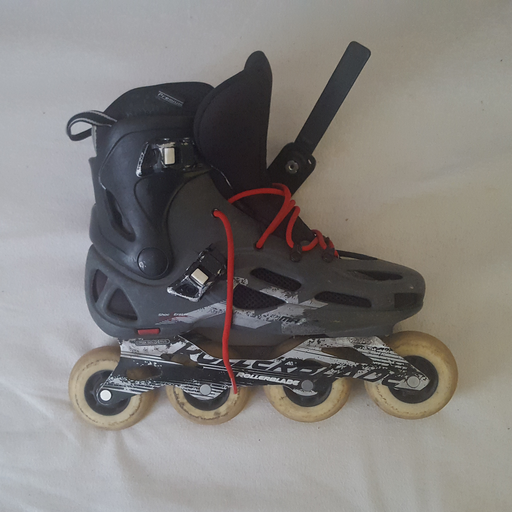
\includegraphics[height=3cm]{images/roller.png}}

\section{Conclusion}
	Le résultat obtenu, bien qu'imprécis permet ensuite, en combinant les silhouettes obtenues de plusieurs points de vues, de reconstituer le modèle 3D de l'objet. On a vu comment numpy pouvait permettre par la vectorisation (virtuelle), d'effectuer des opérations complexes sur des millions de données. L'optimisation spatiale et temporelle rigoureuse permet de mener à bien des calculs complexes (transformée de Fourier) en un temps raisonnable ($\approx 45s$)

\end{multicols}


\noindent\begin{tabular}{|c|p{0.125\textwidth}|p{0.5\textwidth}|p{0.1\textwidth}|p{0.125\textwidth}|}
	\hline
	& Opération & Description & Paramètres & Resultats \\ \hline
	1 & Convertion espace LAB & \vspace{0.01cm}$(L = \frac{R + G + B}{2})$ code l'intensité, $(A = \frac{G - R + 1}{2})$ et $(B = \frac{G - B + 1}{2})$ la couleur. Cette espace est plus relevant pur détecter les bordures d'objet & & \smash{\raisebox{-\height}{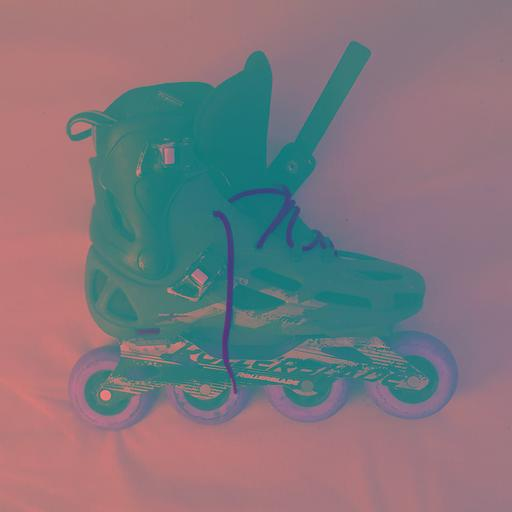
\includegraphics[height=2cm]{images/roller_lab.jpg}}}\vspace{2cm} \\ \hline
	2 & Calcul des composantes de texture & On réalise la convolution du voisinage de chaque pixel par une gaussienne d'orientation et d'écart type variables. On calcul pour cela la transformée de Fourier de chaque voisinage & $\sigma = 4$ \;\; 4 directions & \smash{\raisebox{-\height}{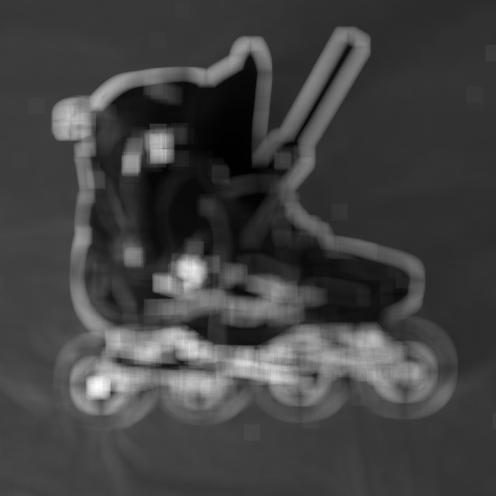
\includegraphics[height=2cm]{images/roller_resp.jpg}}}\vspace{2cm} \\ \hline
	3 & Filtrage & On filtre toutes les composantes par des filtres de Canny (dérivée d'une gaussienne) d'orientation et d'écart type variables. & $\sigma \in \{1,2\}$, 8 directions & \smash{\raisebox{-\height}{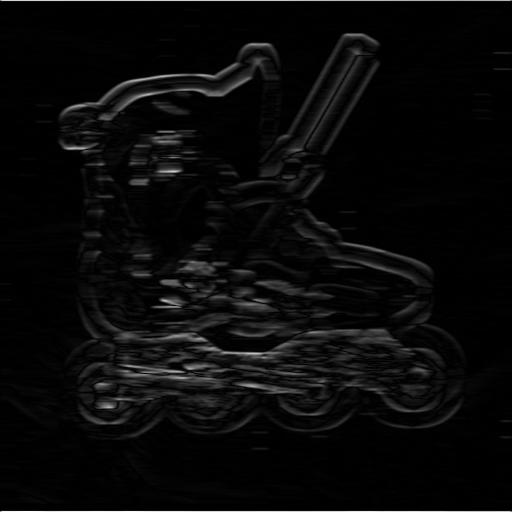
\includegraphics[height=2cm]{images/roller_filtered.jpg}}}\vspace{2cm} \\ \hline
	4 & Lissage parabolique & On approxime le voisinage de chaque pixel par une parabole $(ax^2 + bx + c)$ par la méthode des moindres carrés. On remplace l'image par l'image lissée : $I = \frac{c^+}{\text{distance au max local}} = c^+ \cdot \frac{2a^+}{|b|}$ & 8 directions & \smash{\raisebox{-\height}{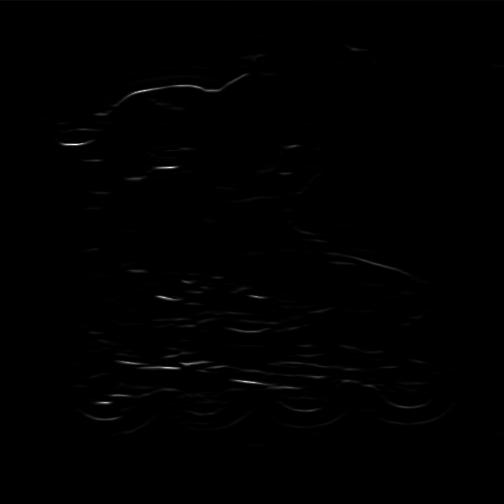
\includegraphics[height=2cm]{images/roller_localised.jpg}}}\vspace{2cm} \\ \hline
	5 & Sommation des réponses & On somme les 20 composantes obtenues $[(2 \text{couleurs} + 4 \text{orientation} * 2 \text{couleurs}) * 2 \text{écart type}]$ en les pondérants par des coefficients piochés dans la littérature. & coefficients de sommations & \smash{\raisebox{-\height}{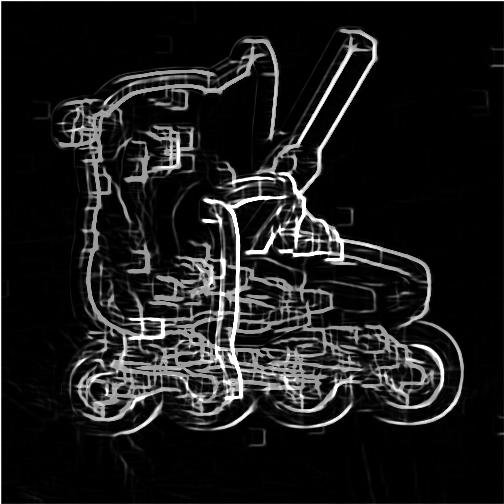
\includegraphics[height=2cm]{images/roller_res.jpg}}}\vspace{2cm} \\ \hline
	6 & Seuillage & On seuille l'image pour obtenir une image binaire & $\text{seuil} = 0.2$ & \smash{\raisebox{-\height}{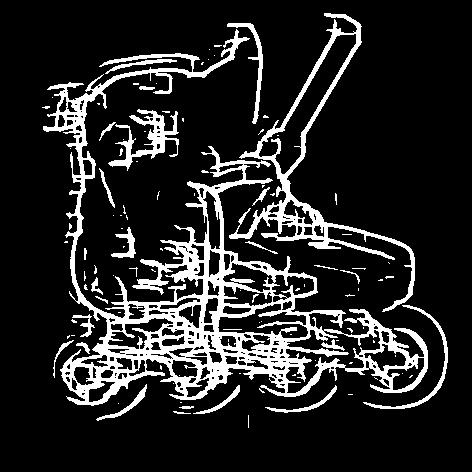
\includegraphics[height=2cm]{images/roller_bin.jpg}}}\vspace{2cm} \\ \hline
	7 & Opérations topologiques & On erode (tous les pixels non entourés sont supprimés) puis on dilate (tous les voisins des pixels sont allumés) successivement afin de fermer le contour de l'image & filtres de fermeture & \smash{\raisebox{-\height}{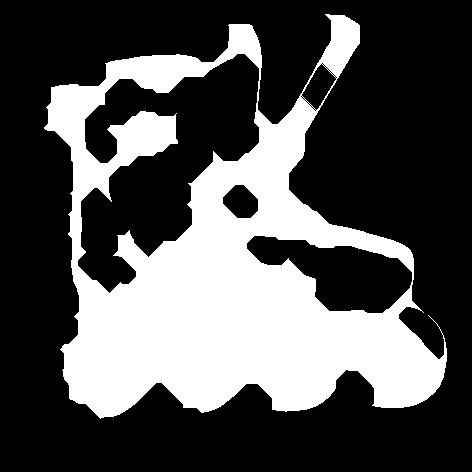
\includegraphics[height=2cm]{images/roller_closedbin.jpg}}}\vspace{2cm} \\ \hline
	8 & Approximation polygonale & On approxime le contour extérieur de l'objet par un polygone en séparant récursivement les segment d'un polygone jusqu'a atteindre un seuil d'approximation (distance maximale polygone-contour) & seuille d'approximation : 10 pixels & \smash{\raisebox{-\height}{
\includegraphics[height=2cm]{images/roller_poly.jpg}}}\vspace{2cm} \\
	\hline
\end{tabular}

\end{document}
